\chapter{Methodology}

The main focus of this chapter is to explain the methods used, discuss the theory behind them as well as the underlying assumptions. 

\section{Benford's Law Formulation}

The relative frequency of a leading digit approaches 

\begin{equation}
    \label{BZ-general_first}
\text{P(} X = d_i\text{)}= \log_{10}(1+1/d_i)
\end{equation}

where $d_i \in \{1,\dots,9\}$ for first digit law and $d_i \in \{10,\dots,99\}$ for the first-two digits law or even $d_i \in \{100,\dots,999\}$ for the first-three digits law. When plotted, it resembles nice logarithmic distribution, as seen on figure \ref{fig:FL}.  \cite{Cerqueti2202,Hronova2023,Newcomb1881}

\begin{figure}[h]
    \centering
    \caption{Theoretical frequencies of the first leading digits}
    \label{fig:FL}
    \pgfplotsset{width=8.5cm,compat=1.18}
        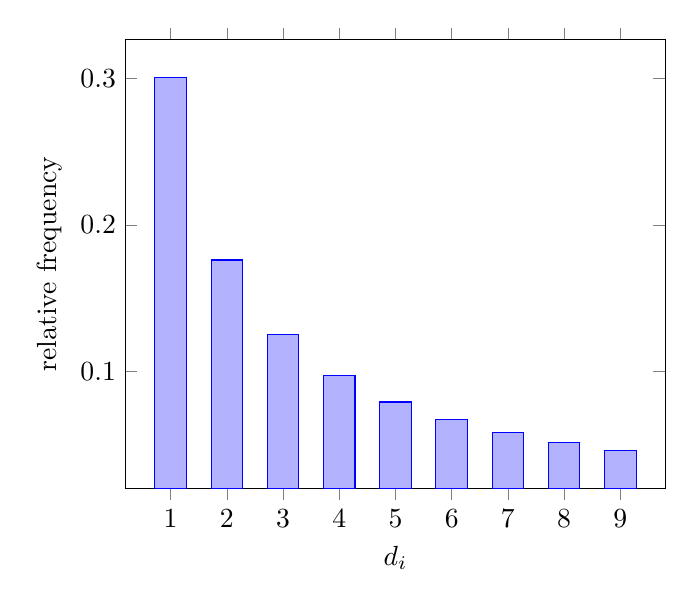
\begin{tikzpicture}
            \begin{axis}[
                ybar,
                bar width=.4cm,
                enlargelimits=0.1,
                ylabel={relative frequency},
                xlabel={$d_i$},
                symbolic x coords={1,2,3,4,5,6,7,8,9},
                xtick=data,
                %nodes near coords,
                %nodes near coords align={vertical},
                ]
            \addplot coordinates {(1,0.3010) (2,0.1761) (3, 0.1249) (4,0.0969) (5,0.0791) (6,0.0669) (7,0.0580) (8,0.0512) (9,0.0458)};
            \end{axis}
        \end{tikzpicture}
    \source{ and processing: author}
\end{figure}

The first leading digit is the one found at the highest order and is non-zero. In the case of the number 124.857, the first digit would be 1, whereas for the number 0.03958, the first digit would be 3. According to Benford's law of the first digit, the theoretical frequencies correspond to the equation \ref{BZ-general_first}, indicating that the digit 1 occurs in the first position with a probability of 0.3, the digit 2 with 0.18, and so forth, with the digit 9 occurring with a probability of only 0.046.

As can be seen in the graph \ref{fig:FL}, the distribution is heavily skewed in favour of the lowest digits. As we move to the second (figure \ref{fig:second-digit-law}) and higher digits, this skew will flatten out significantly until there is no difference between the digits.  \cite{kossovsky2014benford}

This can be described by 

\begin{equation}
    \label{BZ-general_second}
    P(d) = \sum\limits_{k=1}^{9} \log_{10}\left( 1+\frac{1}{10k+d}\right), \quad \text{for } d = 0,1,\dots,9
\end{equation}

as mentioned by \citeauthor{Hronova2023} in \citeyear{Hronova2023}, assuming the independent occurence of the second leading digits. 

\begin{figure}[h]
    \centering
    \caption{Theoretical frequencies of the second leading digits}  
    \label{fig:second-digit-law}
        \pgfplotsset{width=8.5cm,compat=1.18}
            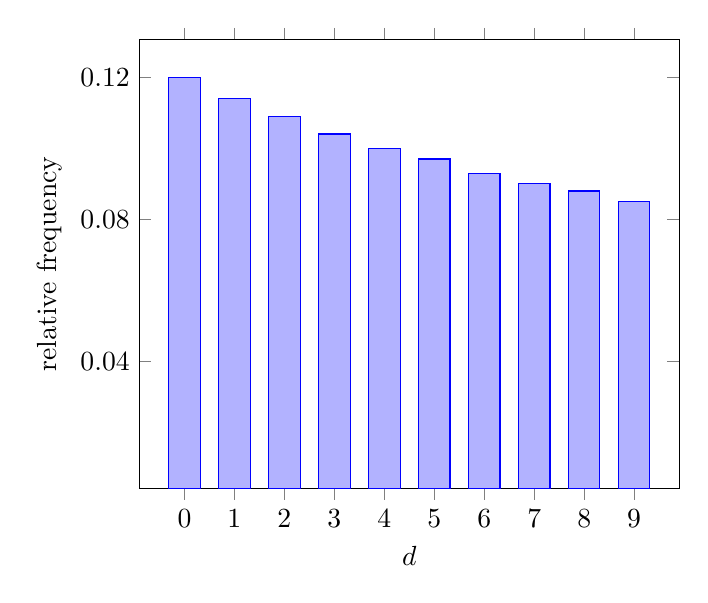
\begin{tikzpicture}
                \begin{axis}[
                    ybar,
                    bar width=.4cm,
                    ymin=0.015,
                    ytick={0.12, 0.08, 0.04},
                    enlargelimits=0.1,
                    ylabel={relative frequency},
                    xlabel={$d$},
                    symbolic x coords={0, 1,2,3,4,5,6,7,8,9},
                    xtick=data,
                    %nodes near coords,
                    %nodes near coords align={vertical},
                    yticklabel style={/pgf/number format/fixed, /pgf/number format/precision=2},
                    ]
                \addplot coordinates {(0,0.12) (1,0.114) (2,0.109) (3, 0.104) (4,0.10) (5,0.097) (6,0.093) (7,0.09) (8,0.088) (9,0.085)};
                \end{axis}
            \end{tikzpicture}
    \source{: \citeauthor{kossovsky2014benford}, \citeyear{kossovsky2014benford}; processing: author}
\end{figure}

The distribution for the second digits is less skewed than that of the first leading digits. Coming to third leading digit, the relative frequencies start to be close to equal as seen on figure \ref{fig:third-digit-law}. \cite{kossovsky2014benford}

This is explained by the following equation 

\begin{equation}
    P(d) = \sum\limits_{d_1=1}^{9} \sum\limits_{d_2=1}^{9} \dots \sum\limits_{d_{k-1}=1}^{9}   \log_{10}\left( 1+\frac{1}{\sum\limits_{i=1}^{k} d_i \cdot 10^{k-i} }\right), \quad \text{for } d_k = 0,1,\dots,9 
\end{equation}

describing third and following position relative frequencies, again with the assumption of independency of digit occurrences. And \uv{\emph{the Benford distribution converges to a uniform
multinomial distribution}} as put in \citeauthor{Hronova2023} in \citeyear{Hronova2023}. 

\begin{figure}[h]
    \centering
    \caption{Theoretical frequencies of the third leading digits}  
    \label{fig:third-digit-law}
    \pgfplotsset{width=8.5cm,compat=1.18}
        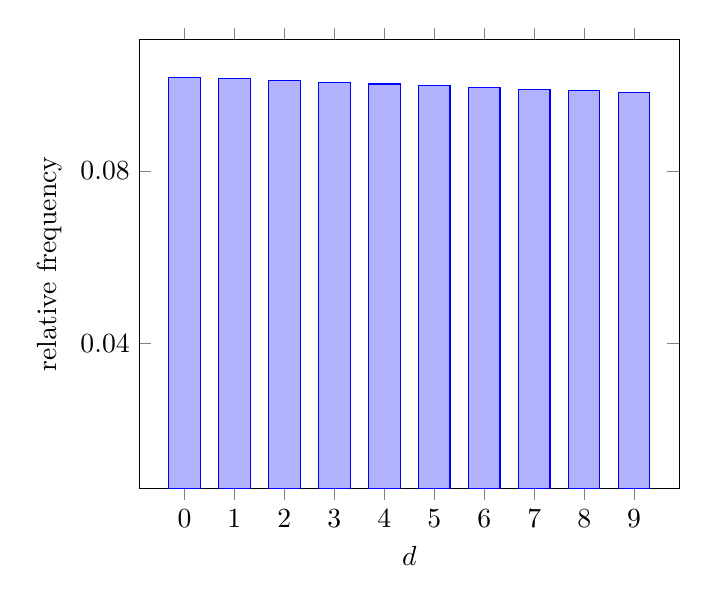
\begin{tikzpicture}
            \begin{axis}[
                ybar,
                bar width=.4cm,
                ymin=0.015,
                ytick={0.12, 0.08, 0.04},
                enlargelimits=0.1,
                ylabel={relative frequency},
                xlabel={$d$},
                symbolic x coords={0,1,2,3,4,5,6,7,8,9},
                xtick=data,
                %nodes near coords,
                %nodes near coords align={vertical},
                yticklabel style={/pgf/number format/fixed, /pgf/number format/precision=2},
                ]
            \addplot coordinates {(0,0.1018) (1,0.1014) (2,0.1010) (3, 0.1006) (4,0.1002) (5,0.0998) (6,0.0994) (7,0.0990) (8,0.0986) (9,0.0983)};
            \end{axis}
        \end{tikzpicture}
    \source{: \citeauthor{kossovsky2014benford}, \citeyear{kossovsky2014benford}; processing: author}
\end{figure}

\begin{koment}
* $\downarrow$ Doplnit jak se delaji tyto navrhovane kroky podle Kossovskyho $\downarrow$ *

First-digits distribution

Second-digits distribution

Combination of the first-two-digits distributions

Combination of the first-three-digits distributions

Combination of the last-two-digits distributions 

Examination of first-order digital development

Examination of second-order digital development

Value repetition test

Summation test  
\end{koment}



\subsection{Selected properties of numbers obeying Benford's Law}

\subsubsection{The Scale Invariance Principle of Benford's Law}

Given a dataset that already behaves according to BL, changing units (multiplying the whole dataset by the same constant), it shall still behave according to BL. Any arithmetic operation applied on the whole dataset, does not change the underlying BL distribution. \cite{kossovsky2014benford, Hronova2023} %section 23 The Scale Invariance Principle 

\subsubsection{Digital Development Pattern}

Dividing the numbers by their orders into intervals such as (0.1,1), (1,10), (10,100) etc., we find that a pattern develops among them - the lower digits like 1 and 2 occur more frequently as the orders increase, while higher digits such as 8 and 9 gradually decrease in frequency. Data based on exponential growth should not be divided into intervals. \cite{kossovsky2014benford} % section 24


\begin{koment}
Comment on the conditions of what the dataset has to meet! 
%Aby BZ platil, musí být čísla - soubor čísel, takzvaně \emph{benfordovský} - dostatečně velký a splňovat podmínku \ref{BZ-podminka} \cite{kossovsky2014benford}. %section 10
\end{koment}

\section{Probability distribution function}

Being one of the defining features of a random variable, the PDF is very important for probabilistic and statistics analyses. It is a non negative function, which integral (sum under its curve) equals to one. 


\section{Hypothesis testing}

\subsection{First and second order errors (alpha beta)}

\subsection{Compliance to BL testing}
To check the compliance of the data to the BL, we can use the $\chi^2$ goodness of fit test. The null hypothesis is that we assume that the empirical distribution follows the theoretical BL distribution. The test criterion is given as such 

\begin{equation}
    \label{chi-sq-test}
    G= n \sum\limits_{d=1}^{9} \frac{(p_d -\pi_d)^2}{\pi_d} 
\end{equation}

\begin{align*}
    \text{where } &\pi_d \text{ is the theoretical frequency under BL distribution} \\
    &p_d \text{ is the empirical frequency from the data} \\ 
    \text{and } &n \text{ is the sample size}
\end{align*} 

as recommended in \citeauthor{Hronova2023}, \citeyear{Hronova2023}.

